%! TeX program = lualatex
\documentclass[a4paper,11pt]{article} 
% packages
\usepackage{censor}
\StopCensoring
\usepackage{fontspec}
\usepackage[most]{tcolorbox}
\setmainfont{EB Garamond}
% for tironian et fallback
% % \directlua{luaotfload.add_fallback
% % ("emojifallback",
% %      {"Noto Serif:mode=harf"}
% % )}
% % \setmainfont{EB Garamond}[RawFeature={fallback=emojifallback}]

\setmonofont[Scale=MatchLowercase]{Deja Vu Sans Mono}
\usepackage[a4paper,left=2cm,right=2cm,top=\dimexpr15mm+1.5\baselineskip,bottom=2cm]{geometry}
\setlength{\parindent}{0pt}

\usepackage{fancyhdr}       % Headers and footers 
\fancyhead[R]{\normalfont \leftmark}
\fancyhead[L]{}
\pagestyle{fancy}

\usepackage{microtype}      % Slightly tweak font spacing for aesthetics
\usepackage{amsmath}
\usepackage[english]{babel} % Language hyphenation and typographical rules
\usepackage{xcolor}
\definecolor{linkblue}{RGB}{0, 64, 128}
\usepackage[final, colorlinks = false, urlcolor = linkblue]{hyperref} 
% \newcommand{\secref}[1]{\textbf{§~\nameref{#1}}}
\newcommand{\secref}[1]{\textbf{§\ref{#1}~\nameref{#1}}}

\usepackage{changepage}     % adjust margins on the fly
\usepackage{algorithm}
\usepackage{algpseudocode}

\usepackage{minted}
\usemintedstyle{algol_nu}

\usepackage{pgfplots}
\pgfplotsset{width=\textwidth,compat=1.9}

\usepackage{caption}
\newenvironment{code}{\captionsetup{type=listing}}{}
\captionsetup[listing]{skip=0pt}
\setlength{\abovecaptionskip}{5pt}
\setlength{\belowcaptionskip}{5pt}

\usepackage[yyyymmdd]{datetime}
\renewcommand{\dateseparator}{--}

\usepackage{enumitem}

\usepackage{titlesec}

\author{Andrew Hayes}

\begin{document}
\begin{titlepage}
    \begin{center}
        \hrule
        \vspace*{0.6cm}
        \censor{\huge \textbf{CT4100}}
        \vspace*{0.6cm}
        \hrule
        \LARGE
        \vspace{0.5cm}
            Information Retrieval
        \vspace{0.5cm}
        \hrule

        \vfill
        \vfill

        \hrule
        \begin{minipage}{0.495\textwidth} 
            \vspace{0.4em}
            \raggedright
            \normalsize 
            Name: Andrew Hayes \\
            E-mail: \href{mailto://a.hayes18@universityofgalway.ie}{\texttt{a.hayes18@universityofgalway.ie}}  \hfill\\   
            Student ID: 21321503 \hfill
        \end{minipage}
        \begin{minipage}{0.495\textwidth} 
            \raggedleft
            \vspace*{0.8cm}
            \Large
            \today
            \vspace*{0.6cm}
        \end{minipage}
        \medskip\hrule 
    \end{center}
\end{titlepage}

\pagenumbering{roman}
\newpage
\tableofcontents
\newpage
\setcounter{page}{1}
\pagenumbering{arabic}

\section{Introduction}
\subsection{Lecturer Contact Details}
\begin{itemize}
    \item   Colm O'Riordan.
    \item   \href{mailto://colm.oriordan@universityofgalway.ie}{\texttt{colm.oriordan@universityofgalway.ie}}.
\end{itemize}

\subsection{Motivations}
\begin{itemize}
    \item   To study/analyse techniques to deal suitably with the large amounts (\& types) of information.
    \item   Emphasis on research \& practice in Information Retrieval.
\end{itemize}

\subsection{Related Fields}
\begin{itemize}
    \item   Artificial Intelligence.
    \item   Database \& Information Systems.
    \item   Algorithms.
    \item   Human-Computer Interaction.
\end{itemize}

\subsection{Recommended Texts}
\begin{itemize}
    \item   \textit{Modern Information Retrieval} -- Riberio-Neto \& Baeza-Yates (several copies in library).
    \item   \textit{Information Retrieval} -- Grossman.
    \item   \textit{Introduction to Information Retrieval} -- Christopher Manning.
    \item   Extra resources such as research papers will be recommended as extra reading.
\end{itemize}

\subsection{Grading}
\begin{itemize}
    \item   Exam: 70\%.
    \item   Assignment 1: 30\%.
    \item   Assignment 2: 30\%.
\end{itemize}

There will be exercise sheets posted for most lecturers; these are not mandatory and are intended as a study aid.

\subsection{Introduction to Information Retrieval}
\textbf{Information Retrieval (IR)} deals with identifying relevant information based on users' information needs, e.g.
web search engines, digital libraries, \& recommender systems. 
It is finding material (usually documents) of an unstructured nature that satisfies an information need within large
collections (usually stored on computers).

\section{Information Retrieval Models}
\subsection{Introduction to Information Retrieval Models}
\textbf{Data collections} are well-structured collections of related items; items are usually atomic with a 
well-defined interpretation.
Data retrieval involves the selection of a fixed set of data based on a well-defined query (e.g., SQL, OQL).
\\\\
\textbf{Information collections} are usually semi-structured or unstructured.
Information Retrieval (IR) involves the retrieval of documents of natural language which is typically not 
structured and may be semantically ambiguous.

\subsubsection{Information Retrieval vs Information Filtering}
The main differences between information retrieval \& information filtering are:
\begin{itemize}
    \item   The nature of the information need.
    \item   The nature of the document set.
\end{itemize}

Other than these two differences, the same models are used.
Documents \& queries are represented using the same set of techniques and similar comparison algorithms are also
used.

\subsubsection{User Role}
In traditional IR, the user role was reasonably well-defined in that a user:
\begin{itemize}
    \item   Formulated a query.
    \item   Viewed the results.
    \item   Potentially offered feedback.
    \item   Potentially reformulated their query and repeated steps.
\end{itemize}

In more recent systems, with the increasing popularity of the hypertext paradigm, users usually intersperse 
browsing with the traditional querying.
This raises many new difficulties \& challenges.

\subsection{Pre-Processing}
\textbf{Document pre-processing} is the application of a set of well-known techniques to the documents \& queries 
prior to any comparison.
This includes, among others:
\begin{itemize}
    \item   \textbf{Stemming:} the reduction of words to a potentially common root.
            The most common stemming algorithms are Lovin's \& Porter's algorithms.
            E.g. \textit{computerisation},
            \textit{computing}, \textit{computers} could all be stemmed to the common form \textit{comput}.
    \item   \textbf{Stop-word removal:} the removal of very frequent terms from documents, which add little to the 
            semantics of meaning of the document.
    \item   \textbf{Thesaurus construction:} the manual or automatic creation of thesauri used to try to identify 
            synonyms within the documents.
\end{itemize}

\textbf{Representation} \& comparison technique depends on the information retrieval model chosen.
The choice of feedback techniques is also dependent on the model chosen.

\subsection{Models}
Retrieval models can be broadly categorised as:
\begin{itemize}
    \item   Boolean:
            \begin{itemize}
                \item   Classical Boolean.
                \item   Fuzzy Set approach.
                \item   Extended Boolean.
            \end{itemize}

    \item   Vector:
            \begin{itemize}
                \item   Vector Space approach.
                \item   Latent Semantic indexing.
                \item   Neural Networks.
            \end{itemize}

    \item   Probabilistic:
            \begin{itemize}
                \item   Inference Network.
                \item   Belief Network.
            \end{itemize}
\end{itemize}

We can view any IR model as being comprised of:
\begin{itemize}
    \item   $D$ is the set of logical representations within the documents.
    \item   $Q$ is the set of logical representations of the user information needs (queries).
    \item   $F$ is a framework for modelling representations ($D$ \& $Q$) and the relationship between $D$ \& $Q$.
    \item   $R$ is a ranking function which defines an ordering among the documents with regard to any query $q$.
\end{itemize}

We have a set of index terms:
$$
t_1, \dots , t_n
$$

A \textbf{weight} $w_{i,j}$ is assigned to each term $t_i$ occurring in the $d_j$.
We can view a document or query as a vector of weights:
$$
\vec{d_j} = (w_1, w_2, w_3, \dots)
$$

\subsection{Boolean Model}
The \textbf{Boolean model} of information retrieval is based on set theory \& Boolean algebra.
A query is viewed as a Boolean expression.
The model also assumes terms are present or absent, hence term weights $w_{i,j}$ are binary \& discrete, i.e., 
$w_{i,j}$ is an element of $\{0, 1\}$.
\\\\
Advantages of the Boolean model include:
\begin{itemize}
    \item   Clean formalism.
    \item   Widespread \& popular.
    \item   Relatively simple
\end{itemize}

Disadvantages of the Boolean model include:
\begin{itemize}
    \item   People often have difficulty formulating expressions, harbours some difficulty in use.
    \item   Documents are considered either relevant or irrelevant; no partial matching allowed.
    \item   Poor performance.
    \item   Suffers badly from natural language effects of synonymy etc.
    \item   No ranking of results.
    \item   Terms in a document are considered independent of each other.
\end{itemize}

\subsubsection{Example}
$$
q = t_1 \land (t_2 \lor (\neg t_3))
$$

\begin{minted}[linenos, breaklines, frame=single]{sql}
q = t1 AND (t2 OR (NOT t3))
\end{minted}

This can be mapped to what is termed \textbf{disjunctive normal form}, where we have a series of disjunctions 
(or logical ORs) of conjunctions.

$$
q = 100 \lor 110 \lor 111
$$

If a document satisfies any of the components, the document is deemed relevant and returned.

\subsection{Vector Space Model}
The \textbf{vector space model} attempts to improve upon the Boolean model by removing the limitation of binary 
weights for index terms.
Terms can have non-binary weights in both queries \& documents.
Hence, we can represent the documents \& the query as $n$-dimensional vectors.

$$
\vec{d_j} = (w_{1,j}, w_{2,j}, \dots, w_{n,j})
$$
$$
\vec{q} = (w_{1,q}, w_{2,q}, \dots, w_{n,q})
$$

We can calculate the similarity between a document \& a query by calculating the similarity between the vector 
representations of the document \& query by measuring the cosine of the angle between the two vectors.
$$
\vec{a} \cdot \vec{b} = \mid \vec{a} \mid \mid \vec{b} \mid \cos (\vec{a}, \vec{b})
$$
$$
\Rightarrow \cos (\vec{a}, \vec{b}) = \frac{\vec{a} \cdot \vec{b}}{\mid \vec{a} \mid \mid \vec{b} \mid}
$$

We can therefore calculate the similarity between a document and a query as:
$$
\text{sim}(q,d) = \cos (\vec{q}, \vec{d}) = \frac{\vec{q} \cdot \vec{d}}{\mid \vec{q} \mid \mid \vec{d} \mid}
$$

Considering term weights on the query and documents, we can calculate similarity between the document \& query as:
$$
\text{sim}(q,d) =
\frac
{\sum^N_{i=1} (w_{i,q} \times w_{i,d})}
{\sqrt{\sum^N_{i=1} (w_{i,q})^2} \times \sqrt{\sum^N_{i=1} (w_{i,d})^2} }
$$

Advantages of the vector space model over the Boolean model include:
\begin{itemize}
    \item   Improved performance due to weighting schemes.
    \item   Partial matching is allowed which gives a natural ranking.
\end{itemize}

The primary disadvantage of the vector space model is that terms are considered to be mutually independent.

\subsubsection{Weighting Schemes}
We need a means to calculate the term weights in the document and query vector representations.
A term's frequency within a document quantifies how well a term describes a document;
the more frequently a term occurs in a document, the better it is at describing that document and vice-versa.
This frequency is known as the \textbf{term frequency} or \textbf{tf factor}.
\\\\
If a term occurs frequently across all the documents, that term does little to distinguish one document from another.
This factor is known as the \textbf{inverse document frequency} or \textbf{idf-frequency}.
Traditionally, the most commonly-used weighting schemes are know as \textbf{tf-idf} weighting schemes.
\\\\
For all terms in a document, the weight assigned can be calculated as:
$$
w_{i,j} = f_{i,j} \times \log \left( \frac{N}{N_i} \right)
$$
where
\begin{itemize}
    \item   $f_{i,j}$ is the (possibly normalised) frequency of term $t_i$ in document $d_j$.
    \item   $N$ is the number of documents in the collection.
    \item   $N_i$ is the number of documents that contain term $t_i$.
\end{itemize}

\section{Evaluation of IR Systems}
When evaluating an IR system, we need to consider:
\begin{itemize}
    \item   The \textbf{functional requirements}: whether or not the system works as intended.
            This is done with standard testing techniques.
    \item   The \textbf{performance:} 
            \begin{itemize}
                \item   Response time.
                \item   Space requirements.
                \item   Measure by empirical analysis, efficiency of algorithms \& data structures for compression,
                        indexing, etc.
            \end{itemize}
    \item   The \textbf{retrieval performance:} how useful is the system?
            IR is a highly empirical discipline and there is a long history of the evaluation of retrieval performance.
            This is less of an issue in data retrieval systems wherein perfect matching is possible as there exists
            a correct answer.
\end{itemize}

\subsection{Test Collections}
Evaluation of IR systems is usually based on a reference \textbf{test collection} involving human evaluations.
The test collection usually comprises:
\begin{itemize}
    \item   A collection of documents $D$.
    \item   A set of information needs that can be represented as queries.
    \item   A list of relevance judgements for each query-document pair.
\end{itemize}

Issues with using test collections include:
\begin{itemize}
    \item   It can be very costly to obtain relevance judgements.
    \item   Crowd sourcing.
    \item   Pooling approaches.
    \item   Relevance judgements don't have to be binary.
    \item   Agreement among judges.
\end{itemize}

\textbf{TREC (Text REtrieval Conference)} provides a means to empirically test the performance of systems in
different domains by providing \textit{tracks} consisting of a data set \& test problems.
These tracks include:
\begin{itemize}
    \item   \textbf{Ad-hoc retrieval:} different tracks have been proposed to test ad-hoc retrieval including the
            Web track (retrieval on web corpora) and the Million Query track (large number of queries).
    \item   \textbf{Interactive Track}: users interact with the system for relevance feedback.
    \item   \textbf{Contextual Search:} multiple queries over time.
    \item   \textbf{Entity Retrieval:} the task is to retrieve entities (people, places, organisations).
    \item   \textbf{Spam Filtering:} identifying \& filtering out non-relevant or harmful content such as email
            spam.
    \item   \textbf{Question Answering (QA):} the goal is to retrieve precise answers to user questions rather than
            returning entire documents.
    \item   \textbf{Cross-Language Retrieval:} the goal is to retrieve relevant documents in a different language
            from the query.
            Requires machine translation.
    \item   \textbf{Conversational IR:} retrieving information in conversational IR systems.
    \item   \textbf{Sentiment Retrieval:} emphasis on identifying opinions \& sentiments.
    \item   \textbf{Fact Checking:} misinformation track.
    \item   \textbf{Domain-Specific Retrieval:} e.g., genomic data.
    \item   Summarisation Tasks.
\end{itemize}

Relevance is assessed for the information need and not the query.
Because tuning \& optimisation can occur for many IR systems, it is considered good practice to tune on one 
collection and then test on another.
\\\\
Interaction with an IR system may be a one-off query or an interactive session.
For the former, \textit{quality} of the returned set is the important metric, while for interactive systems other
issues have to be considered: duration of the session, user effort required, etc.
These issues make evaluation of interactive sessions more difficult.

\subsection{Precision \& Recall}
The most commonly used metrics are \textbf{precision} \& \textbf{recall}.
\subsubsection{Unranked Sets}
Given a set $D$ and a query $Q$, let $R$ be the set of documents relevant to $Q$.
Let $A$ be the set actually returned by the system.
\begin{itemize}
    \item   \textbf{Precision} is defined as $\frac{|R \cap A|}{|A|} = \frac{\text{relevant retrieved documents}}{\text{all retrieved documents}}$, i.e. what fraction of the retrieved documents are relevant.
    \item   \textbf{Recall} is defined as $\frac{|R \cap A|}{|R|} = \frac{\text{relevant retrieved documents}}{\text{all relevant documents}}$, i.e. what fraction of the relevant documents were returned.
\end{itemize}

Having two separate measures is useful as different IR systems may have different user requirements.
For example, in web search precision is of the greatest importance, but in the legal domain recall is of the greatest
importance.
\\\\
There is a trade-off between the two measures; for example, by returning every document in the set, recall is 
maximised (because all relevant documents will be returned) but precision will be poor (because many irrelevant documents will be returned).
Recall is non-decreasing as the number of documents returned increases, while precision usually decreases as the
number of documents returned increases.

\begin{table}[h!]
    \centering
    \begin{tabular}{|p{0.3\textwidth}|p{0.3\textwidth}|p{0.3\textwidth}|}
        \hline
        & \textbf{Relevant} & \textbf{Non-Relevant} \\
        \hline
        \textbf{Relevant} & True Positive (TP) & False Negative (FN) \\
        \hline
        \textbf{Non-Relevant} & False Positive (FP) & True Negative (TN) \\
        \hline
    \end{tabular}
    \caption{Confusion Matrix of True/False Positives \& Negatives}
\end{table}

$$
\text{Precision } P = \frac{tp}{tp + fp} = \frac{\text{true positives}}{\text{true positives + false positives}}
$$
$$
\text{Recall } R = \frac{tp}{tp + fn} = \frac{\text{true positives}}{\text{true positives + false negatives}}
$$

The \textbf{accuracy} of a system is the fraction of these classifications that are correct:
$$
\text{Accuracy} = \frac{tp + tn}{tp +fp + fn + tn}
$$

Accuracy is a commonly used evaluation measure in machine learning classification work, but is not a very useful
measure in IR; for example, when searching for relevant documents in a very large set, the number of irrelevant
documents is usually much higher than the number of relevant documents, meaning that a high accuracy score is
attainable by getting true negatives by discarding most documents, even if there aren't many true positives. 
\\\\
There are also many single-value measures that combine precision \& recall into one value:
\begin{itemize}
    \item   F-measure.
    \item   Balanced F-measure.
\end{itemize}

\subsubsection{Evaluation of Ranked Results}
In IR, returned documents are usually ranked.
One way of evaluating ranked results is to use \textbf{Precision-Recall plots}, wherein precision is typically
plotted against recall.
In an ideal system, we would have a precision value of 1 for a recall value of 1, i.e., all relevant documents
have been returned and no irrelevant documents have been returned.

\begin{tcolorbox}[colback=gray!10, colframe=black, title=\textbf{Example}]
    Given $|D| = 20$ \& $|R| = 10$ and a ranked list of length 10, let the returned ranked list be:
    $$
    \mathbf{d_1}, \mathbf{d_2}, d_3, \mathbf{d_4}, d_5, d_6, \mathbf{d_7}, d_8, d_9, d_{10}
    $$

    where those in items in bold are those that are relevant.
    \begin{itemize}
        \item   Considering the list as far as the first document: Precision = 1, Recall = 0.1.
        \item   As far as the first two documents: Precision = 1, Recall = 0.2.
        \item   As far as the first three documents: Precision = 0.67, Recall = 0.2.
    \end{itemize}

    We usually plot for recall values = 10\% ... 90\%.
\end{tcolorbox}

We typically calculate precision for these recall values over a set of queries to get a truer measure of a system's
performance:
$$
P(r) = \frac{1}{N} \sum^N_{i=1}P_i(r)
$$

Advantages of Precision-Recall include:
\begin{itemize}
    \item   Widespread use.
    \item   It gives a definable measure.
    \item   It summarises the behaviour of an IR system.
\end{itemize}

Disadvantages of Precision-Recall include:
\begin{itemize}
    \item   It's not always possible to calculate the recall measure effective of queries in batch mode.
    \item   Precision \& recall graphs can only be generated when we have ranking.
    \item   They're not necessarily of interest to the user.
\end{itemize}

Single-value measures for evaluating ranked results include:
\begin{itemize}
    \item   Evaluating precision when every new document is retrieved and averaging precision values.
    \item   Evaluating precision when the first relevant document is retrieved.
    \item   $R$-precision: calculate precision when the final document has been retrieved.
    \item   Precision at $k$ (P@k).
    \item   Mean Average Precision (MAP).
\end{itemize}

Precision histograms are used to compare two algorithms over a set of queries.
We calculate the $R$-precision (or possibly another single summary statistic) of two systems over all queries.
The difference between the two are plotted for each of the queries.

\subsection{User-Oriented Measures}
Let $D$ be the document set, $R$ be the set of relevant documents, $A$ be the answer set returned to the users, 
and $U$ be the set of relevant documents previously known to the user.
Let $AU$ be the set of returned documents previously known to the user.
$$
\text{Coverage} = \frac{|AU|}{|U|}
$$
Let \textit{New} refer to the set of relevant documents returned to the user that were previously unknown to the user.
We can define \textbf{novelty} as:
$$
\text{Novelty} = \frac{|\text{New}|}{|\text{New}| + |AU|}
$$

The issues surrounding interactive sessions are much more difficult to assess.
Much of the work in measuring user satisfaction comes from the field of HCI.
The usability of these systems is usually measured by monitoring user behaviour or via surveys of the user's 
experience.
Another closely related area is that of information visualisation: ow best to represent the retrieved data for a
user etc.

\section{Weighting Schemes}
\subsection{Re-cap}
The \textbf{vector space model} attempts to improve upon the Boolean model by removing the limitation of binary weights for index terms.
Terms can have a non-binary value both in queries \& documents.
Hence, we can represent documents \& queries as $n$-dimensional vectors:
$$
\vec{d_j} = \left( w_{1,j} , w_{2,j} , \dots , w_{n,j} \right)
$$
$$
\vec{q} = \left( w_{1,q} , w_{2,q} , \dots , w_{n,q} \right)
$$

We can calculate the similarity between a document and a query by calculating the similarity between the vector representations.
We can measure this similarity by measuring the cosine of the angle between the two vectors.
We can derive a formula for this by starting with the formula for the inner product (dot product) of two vectors:
\begin{align}
a \cdot b = |a| |b| \cos(a,b) \\
\Rightarrow
\cos(a,b) = \frac{a \cdot b}{|a| |b|}
\end{align}

We can therefore calculate the similarity between a document and a query as:
\begin{align*}
    \text{sim}(\vec{d_j}, \vec{q}) = &\frac{d_j \cdot q}{|d_j| |q|} \\
\Rightarrow
    \text{sim}(\vec{d_j}, \vec{q}) = &\frac{\sum^n_{i=1} w_{i,j} \times w_{i,q}}{\sqrt{\sum^n_{i=1} w_{i,j}^2} \times \sqrt{\sum^n_{i=1} w_{i,q}^2}}
\end{align*}

We need a means to calculate the term weights in the document \& query vector representations.
A term's frequency within a document quantifies how well a term describes a document.
The more frequent a term occurs in a document, the better it is at describing that document and vice-versa.
This frequency is known as the \textbf{term frequency} or \textbf{tf factor}.
\\\\
However, if a term occurs frequently across all the documents, then that term does little to distinguish one document from another.
This factor is known as the \textbf{inverse document frequency} or \textbf{idf-frequency}.
The most commonly used weighting schemes are known as \textbf{tf-idf} weighting schemes
For all terms in a document, the weight assigned can be calculated by:
\begin{align*}
    w_{i,j} = f_{i,j} \times \log \frac{N}{n_i}
\end{align*}
where $f_{i,j}$ is the normalised frequency of term $t_i$ in document $d_j$, $N$ is the number of documents in the collection, and $n_i$ is the number of documents that contain the term $t_i$.
\\\\
A similar weighting scheme can be used for queries.
The main difference is that the tf \& idf are given less credence, and all terms have an initial value of 0.5 which is increased or decreased according to the tf-idf across the document collection (Salton 1983).

\subsection{Text Properties}
When considering the properties of a text document, it is important to note that not all words are equally important for capturing the meaning of a document and that text documents are comprised of symbols from a finite alphabet.
\\\\
Factors that affect the performance of information retrieval include:
\begin{itemize}
    \item   What is the distribution of the frequency of different words?
    \item   How fast does vocabulary size grow with the size of a document collection?
\end{itemize}

These factors can be used to select appropriate term weights and other aspects of an IR system.

\subsubsection{Word Frequencies}
A few words are very common, e.g. the two most frequent words ``the'' \& ``of'' can together account for about 10\% of word occurrences.
Most words are very rare: around half the words in a corpus appear only once, which is known as a ``heavy tailed'' or Zipfian distribution.
\\\\
\textbf{Zipf's law} gives an approximate model for the distribution of different words in a document.
It states that when a list of measured values is sorted in decreasing order, the value of the $n^{\text{th}}$ entry is approximately inversely proportional to $n$.
For a word with rank $r$ (the numerical position of the word in a list sorted in by decreasing frequency) and frequency $f$, Zipf's law states that $f \times r$ will equal a constant.
It represents a power law, i.e. a straight line on a log-log plot.
\begin{align*}
    \text{word frequency} \propto \frac{1}{\text{word rank}}
\end{align*}

\begin{figure}[H]
    \centering
    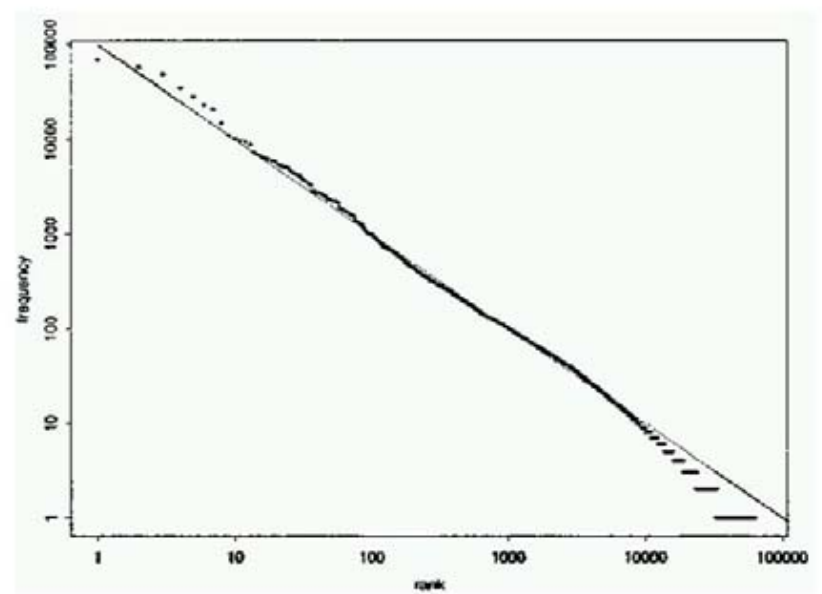
\includegraphics[width=0.8\textwidth]{./images/zipfs_law_brown_corpus.png}
    \caption{Zipf's Law Modelled on the Brown Corpus}
\end{figure}

As can be seen above, Zipf's law is an accurate model excepting the extremes.

\subsection{Vocabulary Growth}
The manner in which the size of the vocabulary increases with the size of the document collection has an impact on our choice of indexing strategy \& algorithms.
However, it is important to note that the size of a vocabulary is not really bounded in the real world due to the existence of mispellings, proper names etc., \& document identifiers.
\\\\
If $V$ is the size of the vocabulary and $n$ is the length of the document collection in word occurrences, then
\begin{align*}
    V = K \cdot n^\beta, \quad 0 < \beta < 1
\end{align*}
where $K$ is a constant scaling factor that determines the initial vocabulary size of a small collection, usually in the range 10 to 100, and $\beta$ is constant controlling the rate at which the vocabulary size increases usually in the range 0.4 to 0.6.

\subsection{Weighting Schemes}
The quality of performance of an IR system depends on the quality of the weighting scheme; we want to assign high weights to those terms with a high resolving power.
tf-idf is one such approach wherein weight is increased for frequently occurring terms but decreased again for those that are frequent across the collection.
The ``bag of words'' model is usually adopted, i.e., that a document can be treated as an unordered collection of words.
The term independence assumption is also usually adopted, i.e., that the occurrence of each word in a document is independent of the occurrence of other words.

\begin{tcolorbox}[colback=gray!10, colframe=black, title=\textbf{``Bag of Words'' / Term Independence Example}]
    If Document 1 contains the text ``Mary is quicker than John'' and Document 2 contains the text ``John is quicker than Mary'', then Document 1 \& Document 2 are viewed as equivalent.
\end{tcolorbox}

However, it is unlikely that 30 occurrences of a term in a document truly carries thirty times the significance of a single occurrence of that term.
A common modification is to use the logarithm of the term frequency:
\begin{align*}
    \text{If } \textit{tf}_{i,d} > 0 \text{:}&   \quad w_{i,d} = 1 + \log(\textit{tf}_{i,d})\\
    \text{Otherwise:}&          \quad w_{i,d} = 0
\end{align*}

\subsubsection{Maximum Term Normalisation}
We often want to normalise term frequencies because we observe higher frequencies in longer documents merely because longer documents tend to repeat the same words more frequently.
Consider a document $d^\prime$ created by concatenating a document $d$ to itself:
$d^\prime$  is no more relevant to any query than document $d$, yet according to the vector space type similarity $\text{sim}(d^\prime, q) \geq \text{sim}(d,q) \, \forall \, q$.
\\\\
The formula for the \textbf{maximum term normalisation} of a term $i$ in a document $d$ is usually of the form
\begin{align*}
\textit{ntf} = a + \left( 1 - a \right) \frac{\textit{tf}_{i,d}}{\textit{tf}\text{max}(d)}
\end{align*}
where $a$ is a smoothing factor which can be used to dampen the impact of the second term.
\\\\
Problems with maximum term normalisation include:
\begin{itemize}
    \item   Stopword removal may have effects on the distribution of terms: this normalisation is unstable and may require tuning per collection.
    \item   There is a possibility of outliers with unusually high frequency.
    \item   Those documents with a more even distribution of term frequencies should be treated differently to those with a skewed distribution.
\end{itemize}

More sophisticated forms of normalisation also exist, which we will explore in the future.

\subsubsection{Modern Weighting Schemes}
Many, if not all of the developed or learned weighting schemes can be represented in the following format
\begin{align*}
    \text{sim}(q,d) = \sum_{t \in q \cap d} \left( \textit{ntf}(D) \times \textit{gw}_t(C) \times \textit{qw}_t(Q) \right)
\end{align*}
where 
\begin{itemize}
    \item   $\textit{ntf}(D)$ is the normalised term frequency in a document.
    \item   $\textit{gw}_t(C)$ is the global weight of a term across a collection.
    \item   $\textit{qw}_t(Q)$ is the query weight of a term in a query $Q$.
\end{itemize}

The \textbf{Okapi BM25} weighting scheme is a standard benchmark weighting scheme with relatively good performance, although it needs to be tuned per collection:
\begin{align*}
    \text{BM25}(Q,D) = \sum_{t \in Q \cap D} \left( \frac{\textit{tf}_{t,D} \cdot \log \left( \frac{N - \textit{df}_t + 0.5}{\textit{df} + 0.5} \right) \cdot \textit{tf}_{t, Q}}{\textit{tf}_{t,D} + k_1 \cdot \left( (1-b) + b \cdot \frac{\textit{dl}}{\textit{dl}_\text{avg}} \right)} \right)
\end{align*}

The \textbf{Pivoted Normalisation} weighting scheme is also as standard benchmark which needs to be tuned for collection, although it has its issues with normalisation:
\begin{align*}
    \text{piv}(Q,D) = \sum_{t \in Q \cap D} \left( \frac{1 + \log \left( 1 + \log \left( \textit{tf}_{t, D} \right) \right)}{(1 - s) + s \cdot \frac{\textit{dl}}{\textit{dl}_\text{avg}}} \right) \times \log \left( \frac{N+1}{\textit{df}_t} \right) \times \textit{tf}_{t, Q}
\end{align*}

The \textbf{Axiomatic Approach} to weighting consists of the following constraints:
\begin{itemize}
    \item   \textbf{Constraint 1:} adding a query term to a document must always increase the score of that document.
    \item   \textbf{Constraint 2:} adding a non-query term to a document must always decrease the score of that document.
    \item   \textbf{Constraint 3:} adding successive occurrences of a term to a document must increase the score of that document less with each successive occurrence.
            Essentially, any term-frequency factor should be sub-linear.
    \item   \textbf{Constraint 4:} using a vector length should be a better normalisation factor for retrieval.
            However, using the vector length will violate one of the existing constraints.
            Therefore, ensuring that the document length factor is used in a sub-linear function will ensure that repeated appearances of non-query terms are weighted less.
\end{itemize}

New weighting schemes that adhere to all these constraints outperform the best known benchmarks.

\section{Relevance Feedback}
We often attempt to improve the performance of an IR system by modifying the user query;
the new modified query is then re-submitted to the system.
Typically, the user examines the returned list of documents and marks those which are relevant.
The new query is usually created via incorporating new terms and re-weighting existing terms.
The feedback from the user is used to re-calculate the term weights.
Analysis of the document set can either be \textbf{local analysis} (on the returned set) or \textbf{global analysis} (on the whole document set).
This feedback allows for the re-formulation of the query, which has the advantage of shielding the user from the task of query reformulation and from the inner details of the comparison algorithm.

\subsection{Feedback in the Vector Space Model}
We assume that relevant documents have similarly weighted term vectors.
$D_r$ is the set of relevant documents returned, $D_n$ is the set of the non-relevant documents returned, and $C_r$ is the set of relevant documents in the entire collection.
If we assume that $C_r$ is known for a query $q$, then the best vector for a query to distinguish relevant documents from non-relevant documents is
\[
    \vec{q} = \left( \frac{1}{\left|C_r\right|} \sum_{d_j \in C_r}d_j \right) - \left( \frac{1}{N - \left|C_r\right|} \sum_{d_j \notin C_r} d_j \right)
\]

However, it is impossible to generate this query as we do not know $C_r$.
We can however estimate $C_r$ as we know $D_r$ which is a subset of $C_r$: the main approach for doing this is the \textbf{Rocchio Algorithm:}
\[
    \overrightarrow{q_{\text{new}}} = \alpha \overrightarrow{q_\text{orginal}} + \frac{\beta}{\left| D_r \right|} \sum_{d_j \in D_r} d_j - \frac{\gamma}{\left| D_n \right|} \sum_{d_j \in D_n}d_j
\]

where $\alpha$, $\beta$, \& $\gamma$ are constants which determine the importance of feedback and the relative importance of positive feedback over negative feedback.
Variants on this algorithm include:
\begin{itemize}
    \item   \textbf{IDE Regular:}
            \[
                \overrightarrow{q_\text{new}} = \alpha \overrightarrow{q_\text{old}} + \beta \sum_{d_j \in D_r} d_j - \gamma \sum_{d_j \in D_n} d_j
            \]

    \item   \textbf{IDE Dec Hi:} (based on the assumption that positive feedback is more useful than negative feedback)
            \[
                \overrightarrow{q_\text{new}} = \alpha \overrightarrow{q_\text{old}} + \beta \sum_{d_j \in D_r} d_j - \gamma \text{MAXNR}(d_j)
            \]
            where $\text{MAXNR}(d_j)$ is the highest ranked non-relevant document.
\end{itemize}

The use of these feedback mechanisms have shown marked improvement in the precision \& recall of IR systems.
Salton indicated in early work on the vector space model that these feedback mechanisms result in an average precision of at least 10\%.
\\\\
The precision-recall is re-calculated for the new returned set, often with respect to the returned document set less the set marked by the user.

\subsection{Pseudo-Feedback / Blind Feedback}
In \textbf{local analysis}, the retrieved documents are examined at query time to determine terms for query expansion.
We typically develop some form of term-term correlation matrix. 
To quantify connection between two terms, we expand the query to include terms correlated to the query terms.

\subsubsection{Association Clusters}
To create an \textbf{association cluster}, first create a matrix $M$;
We can create term $\times$ term matrix to represent the level of association between terms.
This is usually weighted according to
\[
    M_{i,j} = \frac{\text{freq}_{i,j}}{\text{freq}_{i} + \text{freq}_{j} - \text{freq}_{i,j}}
\]

To perform query expansion with local analysis, we can develop an association cluster for each term $t_i$ in the query.
For each term $t_i \in q$ choose the $i^\text{th}$ query term and select the top $N$ values from its row in the term matrix.
For a query $q$, select a cluster for each query term so that $\left| q \right|$ clusters are formed.
$N$ is usually small to prevent generation of very large queries.
We may then either take all terms or just those with the highest summed correlation.

\subsubsection{Metric Clusters}
Association clusters do not take into account the position of terms within documents: \textbf{metric clusters} attempt to overcome this limitation.
Let $\text{dis}(t_i, t_j)$ be the distance between two terms $t_i$ \& $t_j$ in the same document.
If $t_i$ \& $t_j$ are in different documents, then $\text{dis}(t_i, t_j) = \inf$.
We can define the term-term correlation matrix by the following equation, and we can define clusters as before:
\[
    M_{i,j} = \sum_{t_i, t_j \in D_i} \frac{1}{\text{dis}(t_i, t_j)}
\]

\subsubsection{Scalar Clusters}
\textbf{Scalar clusters} are based on comparing sets of words:
if two terms have similar neighbourhoods then there is a high correlation between terms.
Similarity can be based on comparing the two vectors representing the neighbourhoods.
This measure can be used to define term-term correlation matrices and the procedure can continue as before.

\subsection{Global Analysis}
\textbf{Global analysis} is based on analysis of the whole document collection and not just the returned set.
A similarity matrix is created with a similar technique to the method used in the vector space comparison.
We then index each term by the documents in which the term is contained.
It is then possible to calculate the similarity between two terms by taking some measure of the two vectors, e.g. the dot product.
To use this to expand a query, we then:
\begin{enumerate}
    \item   Map the query to the document-term space.
    \item   Calculate the similarity between the query vector and vectors associated with query terms.
    \item   Rank the vectors $\vec{t_i}$ based on similarity.
    \item   Choose the top-ranked terms to add to the query.
\end{enumerate}

\subsection{Issues with Feedback}
The Rocchio \& IDE methods can be used in all vector-based approaches.
Feedback is an implicit component of many other IR models (e.g., neural networks \& probabilistic models).
The same approaches with some modifications are used in information filtering.
Problems that exist in obtaining user feedback include:
\begin{itemize}
    \item   Users tend not to give a high degree of feedback.
    \item   Users are typically inconsistent with their feedback.
    \item   Explicit user feedback does not have to be strictly binary, we can allow a range of values.
    \item   Implicit feedback can also be used, we can make assumptions that a user found an article useful if:
            \begin{itemize}
                \item   The user reads the article.
                \item   The user spends a certain amount of time reading the article.
                \item   The user saves or prints the article.
            \end{itemize}

            However, these metrics are rarely as trustworthy as explicit feedback.
\end{itemize}

\section{Collaborative Filtering}
\textbf{Content filtering} is based solely on matching content of items to user's information needs.
\textbf{Collaborative filtering} collects human judgements and matches people who share the same information needs \& tastes.
Users share their judgements \& opinions.
It echoes the ``word of mouth'' principle.
Advantages of collaborative filtering over content filtering include:
\begin{itemize}
    \item   Support for filtering / retrieval of items where contents cannot be easily analysed in an automated manner.
    \item   Ability to filter based on quality / taste.
    \item   Recommend items that do not contain content the user was expecting.
\end{itemize}

This approach has been successful in a number of domains -- mainly in recommending books/music/films and in e-commerce domains, e.g. Amazon, Netflix, Spotify, ebay, etc.
It has also been applied to collaborative browsing \& searching.
In fact, it can be applied whenever we have some notion of ``ratings'' or ``likes'' or ``relevance'' of items for a set of users.
\\\\
The data in collaborative filtering consists of \textbf{users} (a set of user identifiers), \textbf{items} (a set of item identifiers), \& \textbf{ratings by users of items} (numeric values in some pre-defined range).
We can usually view this as a user-by-item matrix.

\begin{figure}[H]
    \centering
    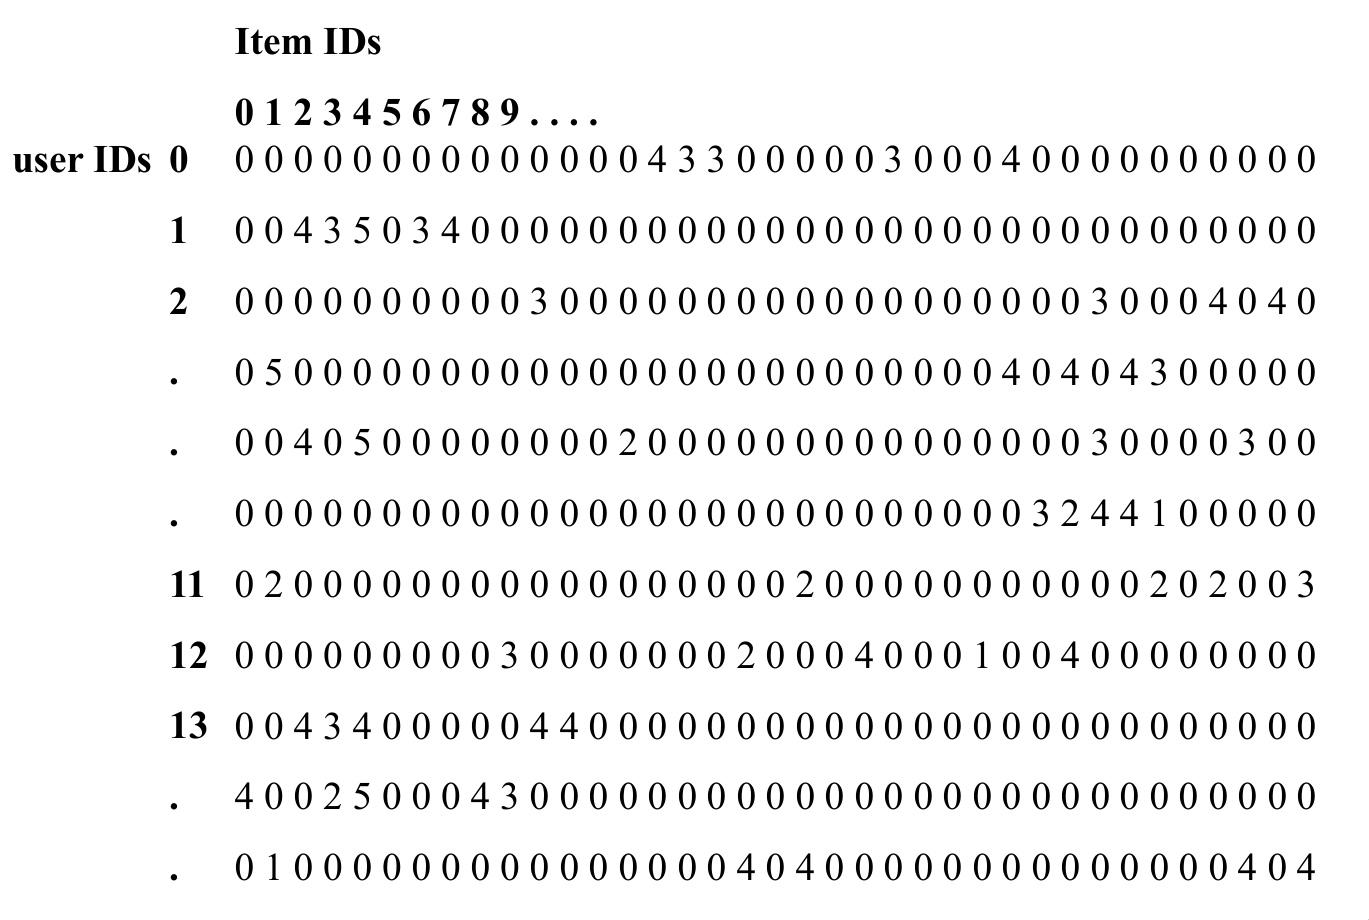
\includegraphics[width=0.8\textwidth]{./images/userbyitemmatrix.png}
    \caption{User-By-Item Matrix Example (ratings from 1 to 5; 0 indicates no rating)}
\end{figure}

With \textbf{explicit ratings}, the user usually provides a single numeric value, although the user maybe unwilling to supply many explicit ratings.
\textbf{Universal queries} are when a gauge set of items is presented to the user for rating.
Choosing a good gauge set is an open question.
\textbf{User-selected queries} are when the user chooses which items to rate (often leaving a sparse ratings matrix with many null values).
\\\\
\textbf{Implicit ratings} are when the user's recommendation is obtained from purchase records, web logs, time spent reading an item, etc.
This implicit rating is usually mapped to some numeric scale.
\\\\
For \textbf{user-user recommendation} approaches, there are three general steps:
\begin{enumerate}
    \item   \textbf{Calculate user correlation:} Find how \textit{similar} each user is to every other user.
    \item   \textbf{Select neighbourhood:} form groups or \textit{neighbourhoods} of users who are similar. 
    \item   \textbf{Generate prediction:} in each group, \textit{make recommendations} based on what other users in the group have rated.
\end{enumerate}

\subsection{Step 1: Calculate User Correlation}
Some approaches for finding how similar each user is to every other user include:
\begin{itemize}
    \item   Pearson correlation.
    \item   Constrained Pearson correlation.
    \item   The Spearman rank correlation.
    \item   Vector similarity.
\end{itemize}

\subsubsection{Pearson Correlation}
\textbf{Pearson correlation} is when a weighted average of deviations from the neighbour's mean is calculated.
\[
    w_{a,u} = \frac{\sum^m_{i=1} (r_{a,i} - \overline{r}_a) \times (r_{u,i} - \overline{r}_u)}
    {\sqrt{\sum^m_{i=1} (r_{u,i} - \overline{r}_u)^2} \times \sqrt{\sum^m_{i=1}(r_{a,i} - \overline{r}_a})^2}
\]
where for $m$ items:
\begin{itemize}
    \item   $r_{a,i}$ is the rating of a user $a$ for an item $i$.
    \item   $r_a$ is the average rating given by a user $a$.
    \item   $r_{u,i}$ is the rating of user $u$ for item $i$.
    \item   $r_u$ is the average rating given by user $u$.
\end{itemize}

\subsubsection{Vector Similarity}
\textbf{Vector similarity} uses the cosine measure between the user vectors (where users are represented by a vector of ratings for items in the data set) to calculate correlation.

\subsection{Step 2: Select Neighbourhood}
Some approaches for forming groups or \textbf{neighbourhoods} of users who are similar include:
\begin{itemize}
    \item   \textbf{Correlation thresholding:} all neighbours with absolute correlations greater than a specified threshold are selected, say 0.7 if correlations in range 0 to 1.
    \item   \textbf{Best-$n$ correlations:} the best $n$ correlates are chosen.
\end{itemize}

A large neighbourhood can result in low-precision results, while a small neighbourhood can result in few or now predictions.

\subsection{Step 3: Generate Predictions}
For some user (the active user) in a group, make recommendations based on what other users inthe group have rated which the active user has not rated.
Approaches for doing so include:
\begin{itemize}
    \item   \textbf{Compute the weighted average} of the user rating using the correlations as the weights.
            This weighted average approach makes an assumption that all users rate items with approximately the same distribution.
    \item   \textbf{Compute the weighted mean} of all neighbours' ratings.
            Rather than take the explicit numeric value of a rating, a rating's strength is interpreted as its distance from a neighbour's mean rating.
            This approach attempts to account for the lack of uniformity in ratings.

            \[
                P_{a,i} = \bar{r}_a + \frac{\sum^n_{u=1} (r_{u,i - \bar{r}_u}) \times w_{a,u}}{\sum^n_{u=1} w_{a,u}}
            \]
            where for $n$ neighbours:
            \begin{itemize}
                \item   $\bar{r}_a$ is the average rating given by active user $a$.
                \item   $r_{u,i}$ is the rating of user $u$ for item $i$.
                \item   $w_{a,u}$ is the similarity between user $u$ and $a$.
            \end{itemize}
\end{itemize}

Note that the Pearson Correlation formula does not explicitly take into account the number of co-rated items by users.
Thus it is possible to get a high correlation value based on only one co-rated item.
Often, the Pearson Correlation formula is adjusted to take this into account.

\subsection{Experimental Approach for Testing}
A known collection of ratings by users over a range of items is decomposed into two disjoint subsets.
The first set (usually the larger) is used to generate recommendations for items corresponding to those in the smaller set.
These recommendations are then compared to the actual ratings in the second subset.
The accuracy \& coverage of a system can thus be ascertained.

\subsubsection{Metrics}
The main metrics used to test the predictions produced are:
\begin{itemize}
    \item   \textbf{Coverage:} a measure of the ability of the system to provide a recommendation on a given item.
    \item   \textbf{Accuracy:} a measure of the correctness of the recommendations generated by the system.
\end{itemize}

\textbf{Statistical accuracy metrics} are usually calculated by comparing the ratings generated by the system to user-provided ratings.
The accuracy is usually presented as the mean absolute error (\textbf{MAE}) between ratings \& predictions.
\\\\
Typically, the value of the rating is not that important: it is more important to know if the rating is a useful or a non-useful rating.
\textbf{Decision support accuracy metrics} measure whether the recommendation is actually useful to the user.
Many other approaches also exist, including:
\begin{itemize}
    \item   Machine learning approaches.
            \begin{itemize}
                \item   Bayesian models.
                \item   Clustering models.
            \end{itemize}
    \item   Models of how people rate items.
    \item   Data mining approaches.
    \item   Hybrid models which combine collaborative filtering with content filtering.
    \item   Graph decomposition approaches.
\end{itemize}

\subsection{Collaborative Filtering Issues}
\begin{itemize}
    \item   \textbf{Sparsity of Matrix:} in a typical domain, there would be many users \& many items but any user would only have rated a small fraction of all items in the dataset.
            Using a technique such as \textbf{Singular Value Decomposition (SVD)}, the data space can be reduced, and due to this reduction a correlation may be found between similar users who do not have overlapping ratings in the original matrix of ratings.

    \item   \textbf{Size of Matrix:} in general, the matrix is very large, which can affect computational efficiency.
            SVD has been used to improve scalability by dimensionality reduction.

    \item   \textbf{Noise in Matrix:} we need to consider how would a user's ratings change for items and how to model time dependencies; are all ratings honest \& reliable?

    \item   \textbf{Size of Neighbourhood:} while the size of the neighbourhood affects predictions, there is no way to know the ``right'' size.
             Need to consider whether visualisation of the would neighbourhood help, whether summarisation of the main themes/feature of neighbourhoods help.

    \item   \textbf{How to Gather Ratings:} new users, new items: perhaps use weighted average of global mean \& users or items.
            What if the user is not similar to others?
\end{itemize}

\subsection{Combining Content \& Collaborative Filtering}
For most items rated in a collaborative filtering domain, content information is also available:
\begin{itemize}
    \item   Books: author, genre, plot summary, language, etc.
    \item   Music: artist, genre, sound samples, etc.
    \item   Films: director, genre, actors, year, country, etc.
\end{itemize}

Traditionally, content is not used in collaborative filtering, although it could be.
\\\\
Different approaches may suffer from different problems, so can consider combining multiple approaches.
We can also view collaborative filtering as a machine learning classification problem: for an item, do we classify it as relevant to a user or not?
\\\\
Much recent work has been focused on not only giving a recommendation, but also attempting to explain the recommendation to the user.
Questions arise in how best to ``explain'' or visualise the recommendation.

\section{Learning in Information Retrieval}
Many real-world problems are complex and it is difficult to specify (algorithmically) how to solve many of these problems.
Learning techniques are used in many domains to find solutions to problems that may not be obvious or clear to human users.
In general, machine learning involves searching a large space of potential hypotheses or potential solutions to find the hypotheses/solution that best \textit{explains} or \textit{fits} a set of data and any prior knowledge, or is the best solution, or the solution that we can say learns if it improves the performance. 
\\\\
Machine learning techniques require a training stage before the learned solution can be used on new previously unseen data.
The training stage consists of a data set of examples which can either be:
\begin{itemize}
    \item   \textbf{Labelled} (supervised learning).
    \item   \textbf{Unlabelled} (unsupervised learning).
\end{itemize}

An additional data set must also be used to test the hypothesis/solution.
\\\\
\textbf{Symbolic knowledge} is represented in the form of the symbolic descriptions of the learned concepts, e.g., production rules or concept hierarchies.
\textbf{Sub-symbolic knowledge} is represented in sub-symbolic form not readable by a user, e.g., in the structure, weights, \& biases of the trained network.

\subsection{Genetic Algorithms}
\textbf{Genetic algorithms} are inspired by the Darwinian theory of evolution:
at each step of the algorithm, the best solutions are selected while the weaker solutions are discarded.
It uses operators based on crossover \& mutation as the basis of the algorithm to sample the space of solutions.
The steps of a genetic algorithm are as follows: first, create a random population. 
Then, while a solution has not been found:
\begin{enumerate}
    \item   Calculate the fitness of each individual.
    \item   Select the population for reproduction:
            \begin{enumerate}[label=\roman*.]
                \item   Perform crossover.
                \item   Perform mutation.
            \end{enumerate}
    \item   Repeat.
\end{enumerate}

\tikzstyle{process} = [rectangle, minimum width=2cm, minimum height=1cm, text centered, draw=black]
\tikzstyle{arrow} = [thick,->,>=stealth]
% \usetikzlibrary{patterns}

\begin{figure}[H]
    \centering
    \begin{tikzpicture}[node distance=2cm]
        \node (reproduction)    [process] at (0, 2.5)  {Reproduction, Crossover, Mutation};
        \node (population)      [process] at (-2.5, 0) {population};
        \node (fitness)         [process] at (0, -2.5) {Calculate Fitness};
        \node (select)          [process] at (2.5, 0)  {Select Population};

        \draw [arrow] (population) -- (fitness);
        \draw [arrow] (fitness) -- (select);
        \draw [arrow] (select) -- (reproduction);
        \draw [arrow] (reproduction) -- (population);
    \end{tikzpicture}
    \caption{Genetic Algorithm Steps}
\end{figure}

Traditionally, solutions are represented in binary.
A \textbf{phenotype} is the decoding or manifestation of a \textbf{genotype} which is the encoding or representation of a phenotype.
We need an evaluation function which will discriminate between better and worse solutions.
\begin{tcolorbox}[colback=gray!10, colframe=black, title=\textbf{Crossover Examples}]
Example  of one-point crossover:
\texttt{11001\underline{011}} and \texttt{11011\underline{111}} gives \texttt{11001\underline{111}} and \texttt{11011\underline{011}}.
\\\\
Example of $n$-point crossover: \texttt{\underline{110}110\underline{11}0} and \texttt{0001001000} gives \texttt{\underline{110}100\texttt{11}00} and \texttt{000\underline{110}10\underline{01}}.
\end{tcolorbox}

\textbf{Mutation} occurs in the genetic algorithm at a much lower rate than crossover.
It is important to add some diversity to the population in the hope that new better solutions are discovered and therefore it aids in the evolution of the population.
\begin{tcolorbox}[colback=gray!10, colframe=black, title=\textbf{Mutation Example}]
Example  of mutation: \texttt{1\underline{1}001001} $\rightarrow$ \texttt{1\underline{0}001001}.
\end{tcolorbox}

There are two types of selection:
\begin{itemize}
    \item   \textbf{Roulette wheel selection:} each sector in the wheel is proportional to an individual's fitness.
            Select $n$ individuals by means of $n$ roulette turns.
            Each individual is drawn independently.
        \item   \textbf{Tournament selection:} a number of individuals are selected at random with replacement from the population.
                The individual with the best score is selected.
                This is repeated $n$ times.
\end{itemize}

Issues with genetic algorithms include:
\begin{itemize}
    \item   Choice of representation for encoding individuals.
    \item   Definition of fitness function.
    \item   Definition of selection scheme.
    \item   Definition of suitable genetic operators.
    \item   Setting of parameters:
            \begin{itemize}
                \item   Size of population.
                \item   Number of generations.
                \item   Probability of crossover.
                \item   Probability of mutation.
            \end{itemize}
\end{itemize}

\begin{tcolorbox}[colback=gray!10, colframe=black, title=\textbf{Case Study 1: Application of Genetic Algorithms to IR}]
    The effectiveness of an IR system is dependent on the quality of the weights assigned to terms in documents.
    We have seen heuristic-based approaches \& their effectiveness and we've seen axiomatic approaches that could be considered.
    \\\\
    Why not learn the weights?
    We have a definition of relevant \& non-relevant documents; we can use MAP or precision@$k$ as fitness.
    Each genotype can be a set of vectors of length $N$ (the size of the lexicon).
    Set all rates randomly initially.
    Run the system with a set of queries to obtain fitness; select good chromosomes; crossover; mutate.
    Effectively searching the landscape for weights to give a good ranking.
\end{tcolorbox}


\subsection{Genetic Programming}
\textbf{Genetic programming} applies the approach of the genetic algorithm to the space of possible computer programs.
``Virtually all problems in artificial intelligence, machine learning, adaptive systems, \& automated learning can be recast as a search for a computer program.
Genetic programming provides a way to successfully conduct the search for a computer program in the space of computer programs.'' -- Koza.
\\\\
A random population of solutions is created which are modelled in a tree structure with operators as internal nodes and operands as leaf nodes.


\begin{figure}[H]
    \centering
    \usetikzlibrary{trees}
    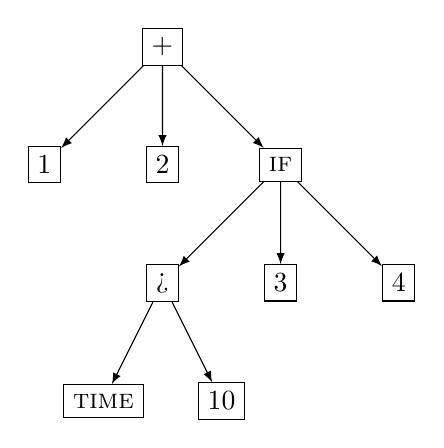
\begin{tikzpicture}
        [
        every node/.style = {draw, shape=rectangle, align=center},
        level distance = 1.5cm,
        sibling distance = 1.5cm,
        edge from parent/.style={draw,-latex}
        ]
        \node {+}
            child { node {1} }
            child { node {2} }
            child { node {\textsc{if}}
                child { node {>}
                    child { node {\textsc{time}} }
                    child { node {10} }
                }
                child { node {3} }
                child { node {4} }
            };
    \end{tikzpicture}
    \caption{\texttt{(+ 1 2 (IF (> TIME 10) 3 4))}}
\end{figure}

\begin{figure}[H]
    \centering
    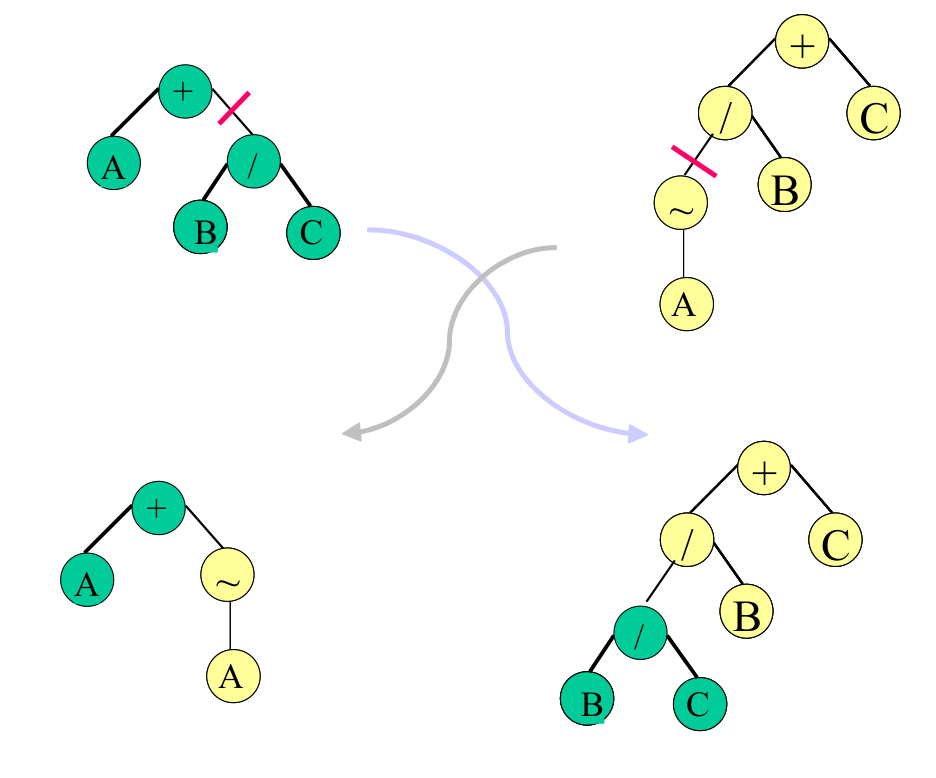
\includegraphics[width=0.4\textwidth]{./images/crossover.png}
    \caption{Crossover Example}
\end{figure}

\begin{figure}[H]
    \centering
    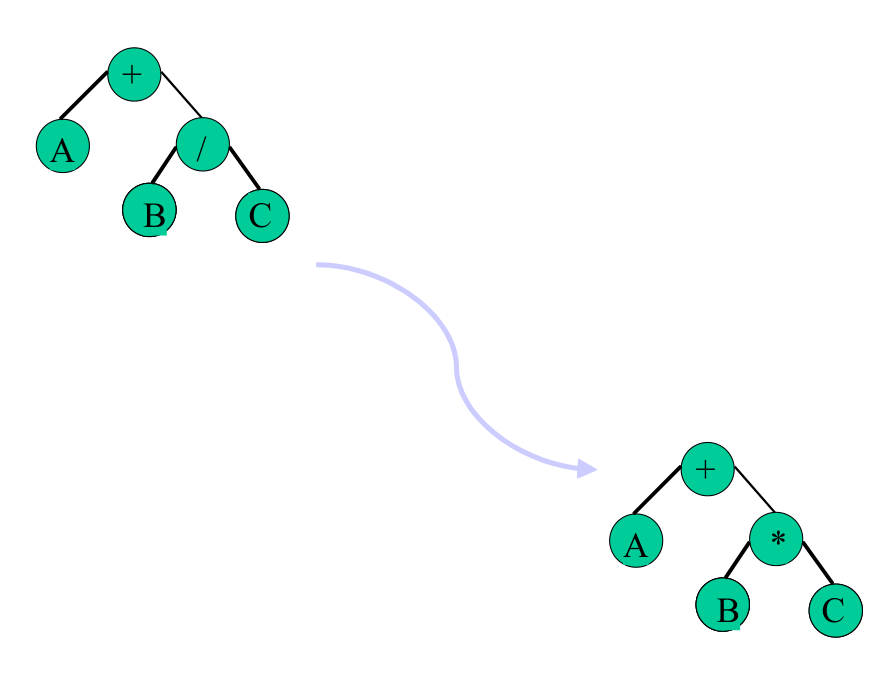
\includegraphics[width=0.4\textwidth]{./images/mutation.png}
    \caption{Mutation Example}
\end{figure}

The genetic programming flow is as follows:
\begin{enumerate}
    \item   Trees are (usually) created at random.
    \item   Evaluate how each tree performs in its environment (using a fitness function).
    \item   Selection occurs based on fitness (tournament selection).
    \item   Crossover of selected solutions to create new individuals.
    \item   Repeat until population is replaced.
    \item   Repeat for $N$ generations.
\end{enumerate}

\subsubsection{Anatomy of a Term-Weighting Scheme}
Typical components of term weighting schemes include:
\begin{itemize}
    \item   Term frequency aspect.
    \item   ``Inverse document'' score.
    \item   Normalisation factor.
\end{itemize}

The search space should be decomposed accordingly.

\subsubsection{Why Separate Learning into Stages?}
The search space using primitive measures \& functions is extremely large;
reducing the search space is advantageous as efficiency is increased.
It eases the analysis of the solutions produced at each stage.
Comparisons to existing benchmarks at each of these stages can be used to determine if the GP is finding novel solutions or variations on existing solutions.
It can then be identified from where any improvement in performance is coming.

\subsubsection{Learning Each of the Three Parts in Turn}
\begin{enumerate}
    \item   Learn a term-discrimination scheme (i.e., some type of idf) using primitive global measures.
            \begin{itemize}
                \item   8 terminals \& 8 functions.
                \item   $T = \{\textit{df}, \textit{cf}, N, V, C, 1, 10, 0.5\}$.
                \item   $F = \{+, \times, \div, -, \text{square}(), \text{sqrt}(), \text{ln}(), \text{exp}()\}$.
            \end{itemize}

    \item   Use this global measure and learn a term-frequency aspect.
            \begin{itemize}
                \item   4 terminals \& 8 functions.
                \item   $T = \{\textit{tf}, 1, 10, 0.4\}$.
                \item   $F = \{+, \times, \div, -, \text{square}(), \text{sqrt}(), \text{ln}(), \text{exp}()\}$.
            \end{itemize}

    \item   Finally, learn a normalisation scheme.
            \begin{itemize}
                \item   6 terminals \& 8 functions.
                \item   $T = \{ \text{dl}, \text{dl}_{\text{avg}}, \text{dl}_\text{dev}, 1, 10, 0.5 \}$.
                \item   $F = \{ +, \times, \div, -, \text{square}(), \text{sqrt}(), \text{ln}(), \text{exp}() \}$.
            \end{itemize}
\end{enumerate}

\begin{figure}[H]
    \centering
    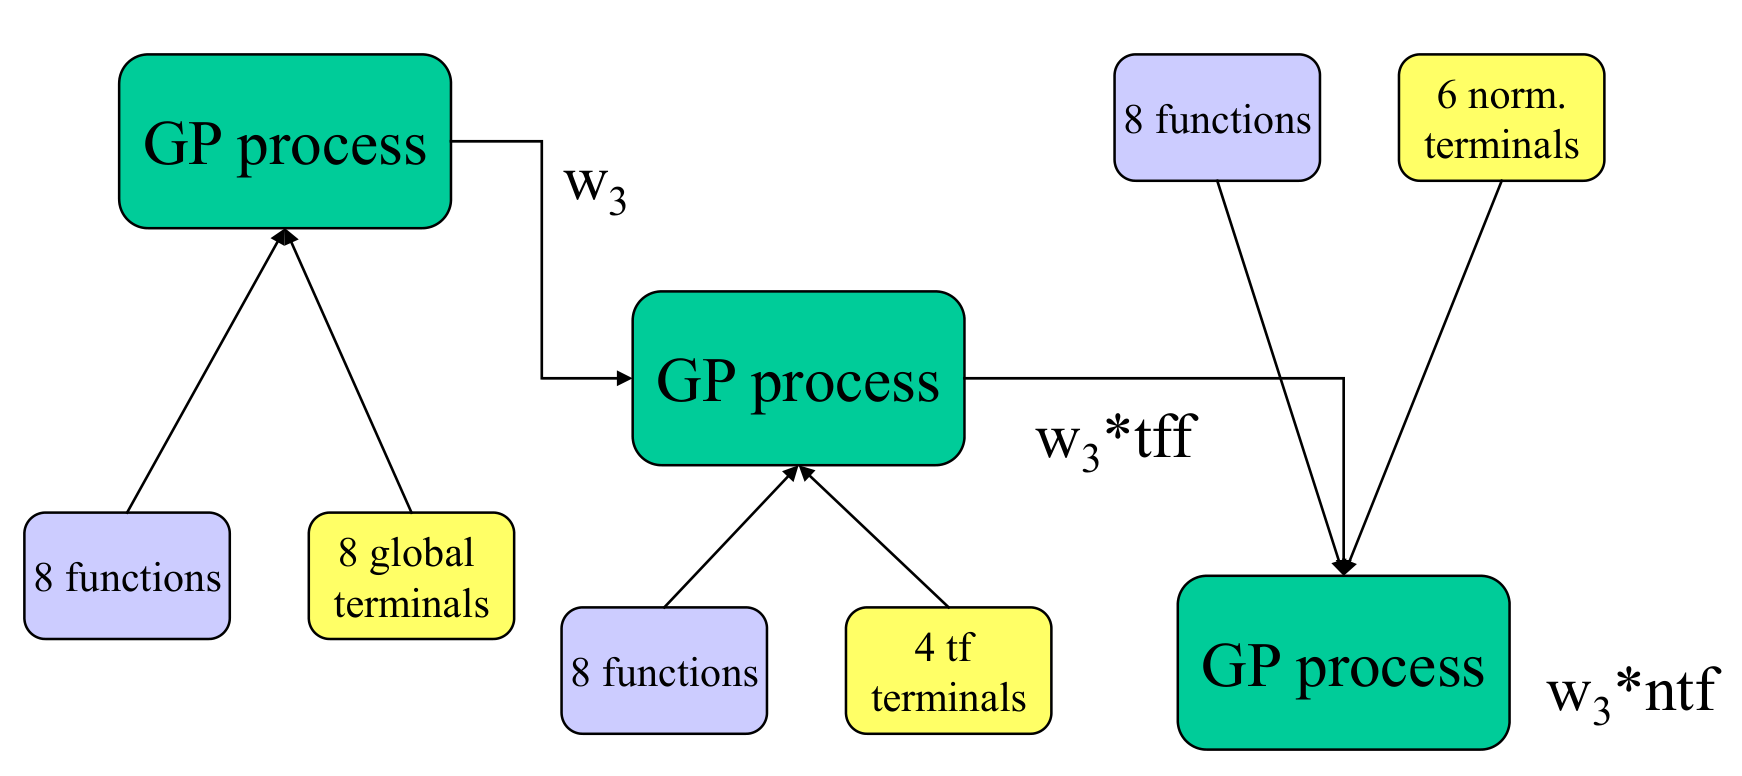
\includegraphics[width=0.6\textwidth]{./images/threestages.png}
    \caption{Learning Each of the Three Stages in Turn}
\end{figure}

\subsubsection{Details of the Learning Approach}
\begin{itemize}
    \item   7 global functions were developed on \~32,000 OHSUMED documents.
            \begin{itemize}
                \item   All validated on a larger unseen collection and the best function taken.
                \item   Random population of 100 for 50 generations.
                \item   The fitness function used was MAP.
            \end{itemize}

    \item   7 tf functions were developed on \~32,000 LATIMES documents.
            \begin{itemize}
                \item   All validated on a larger unseen collection and the best function taken.
                \item   Random population of 200 for 25 generations.
                \item   The fitness function used was MAP.
            \end{itemize}

    \item   7 normalisation functions were developed 3 $\times$ \~ 10,000 LATIMES documents.
            \begin{itemize}
                \item   All validated on a larger unseen collection and the best function taken.
                \item   Random population of 200 for 25 generations.
                \item   Fitness function used was average MAP over the 3 collections.
            \end{itemize}
\end{itemize}

\subsubsection{Analysis}
The global function $w_3$ always produces a positive number:
\[
    w_3 = \sqrt{\frac{\textit{cf}^3_t \cdot N}{\textit{df}^4_t}}
\]


\begin{tcolorbox}[colback=gray!10, colframe=black, title=\textbf{Case Study 1: Application of Genetic Programming to IR}]
    Evolutionary computing approaches include:
    \begin{itemize}
        \item   Evolutionary strategies.
        \item   Genetic algorithms.
        \item   Genetic programming.
    \end{itemize}

    Why genetic programming for IR?
    \begin{itemize}
        \item   Produces a symbolic representation of a solution which is useful for further analysis.
        \item   Using training data, MAP can be directly optimised (i.e., used as the fitness function).
        \item   Solutions produced are often generalisable as solution length (size) can be controlled.
    \end{itemize}
\end{tcolorbox}

Empirical evaluation shows that the evolved scheme outperforms a tuned pivot normalisation scheme and a tuned BM25 scheme.
The evolved scheme is also non-parametric.
The use of primitive atomic measures and basic function types is crucial in allowing the shape of term-weighting functions to evolve.

\subsection{Neural Networks}
Previously, we reviewed the notion of learning in IR and looked at the application of the evolutionary computation approach as a search for solutions in information retrieval.
The advantages were that we had solutions that could be analysed.
However, the usefulness of the solution found is dependent on the usefulness of the primitive features chosen to extract from queries and the documents collection.
\\\\
The dominant learning approach in recent years has been the \textbf{neural} approach.
The neural approach can be seen being applied directly to:
\begin{itemize}
    \item   The information retrieval tasks itself.
    \item   To other related problems/areas that can feed into the IR process.
    \item   Related problems in IR (e.g., query suggestions).
\end{itemize}

Approaches in the domain have been both supervised \& unsupervised.
One of the first approaches to adopt a neural network model can be traced back to the 1980s, with an effectively three-layer network consisting of documents, terms, \& query.
A spreading activation method was used, where query nodes are highlights and propagate to terms which in turn highlight certain documents.


\begin{tcolorbox}[breakable, colback=gray!10, colframe=black, title=\textbf{Case Study: Self-Organising Maps (Kohonen)}]
Self-organising maps are an example of unsupervised learning.
Documents are mapped to 2D space, and dense areas indicate clusters hierarchically.
In the Kohonen approach, documents are mapped to 2D space and each region is characterised / represented by terms.

\begin{figure}[H]
    \centering
    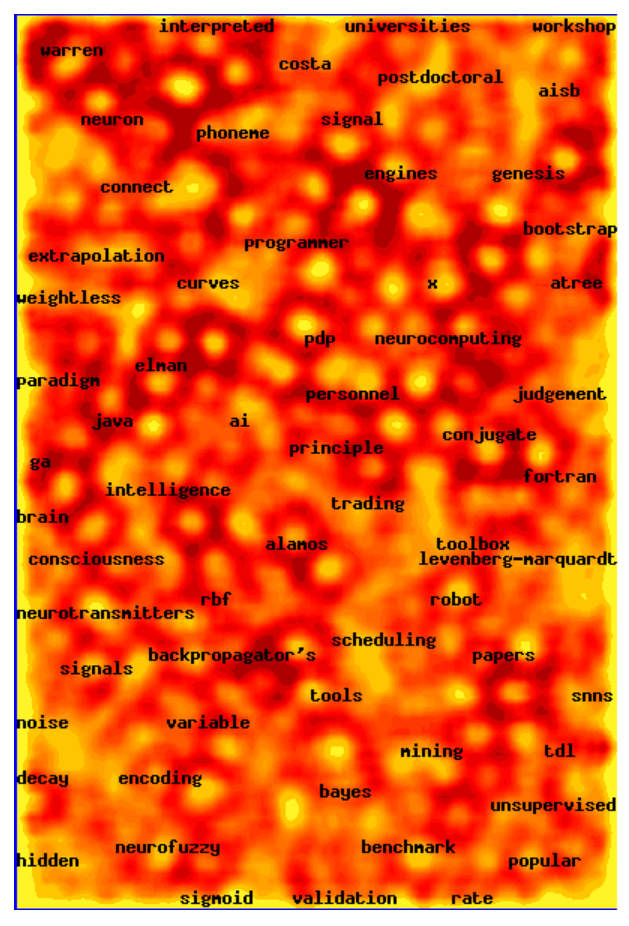
\includegraphics[width=0.4\textwidth]{./images/som.png}
    \caption{A SOM created over a collection of AI-related documents}
\end{figure}

Users can traverse the collection by clicking on an area of the map that is of interest.

\begin{figure}[H]
    \centering
    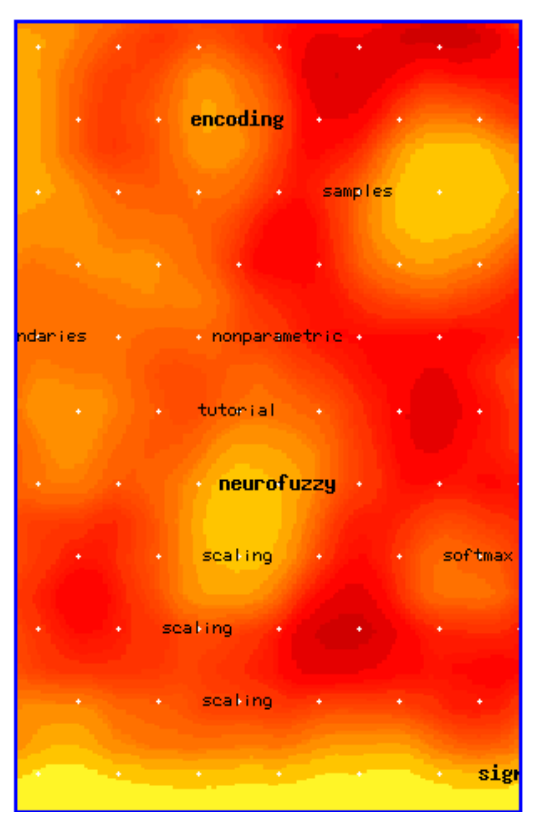
\includegraphics[width=0.4\textwidth]{./images/som1.png}
    \caption{Finally, the user arrives at a list of papers/articles that have been clustered together}
\end{figure}

Kohonen self-organising maps represent a sub-symbolic, neural approach to clustering.
The algorithm takes a set of $n$-dimensional vectors and attempts to map them onto a two-dimensional grid.
The grid comprises of a set of nodes, each of which is assigned an $n$-dimensional vector.
These vectors contain randomly assigned weights.
\\\\
The algorithm is as follows:
\begin{enumerate}
    \item   Select an input vector randomly.
    \item   Identify the grid node which is closest to the input vector: the ``winning node''.
    \item   Adjust the weights on the winning node so that it is closer to the input vector.
    \item   Adjust the weights on nodes near to the winning node so that they are closer to the winning node.
\end{enumerate}

Note:
\begin{itemize}
    \item   The rate of modification of weights decreases over time.
    \item   The size of the neighbourhood affected (near the winning node) decreases over time.
    \item   The resulting clustering of tuples maintains the distance relationship between the input data.
\end{itemize}
\end{tcolorbox}

There has been huge interest in the application of NN models in IR in recent years as there have been several breakthroughs due to the use of neural networks with multiple layers (so-called ``deep architectures'') and the availability of large datasets \& computing power.
Proposed neural models learn representations of language from raw text that can bridge the gap between query \& document vocabulary.
Neural IR is the application of shallow or deep NN to IR tasks.
\\\\
Neural models for IR use vector representations of text and usually contain a large number of parameters that need to be tuned.
ML models with a large set of parameters benefit from large quantities of training data.
Unlike traditional ``learning to rank'' approaches that train over a set of hand-crafted features, more recent NN accept the raw text as input.
Some main steps in classical IR include:
\begin{itemize}
    \item   Generating a representation of the user's query.
    \item   Generating a representation of the documents that captures the ``content'' of the document.
    \item   Generating a ``similarity'' score (comparison).
\end{itemize}

All neural approaches can be classified as to whether they affect the representation of the query, the document, or the comparison.
By inspecting only the query terms, the IR model ignores all evidence of the context provided in the rest of the document: only occurrences of a word are included, and not other terms that capture the same meaning or the same topic.
Traditional IR models have also used dense vector representations of terms \& documents.
Many neural representations have commonalities with these traditional approaches.

\subsection{Query Representation}
Types of vector representations include:
\begin{itemize}
    \item   One-Hot representations: akin to what we have seen thus far, in that each term is represented by one value.
    \item   Distributed representation: typically a real-valued vector which attempts to better capture the meaning of the terms.
\end{itemize}

NNs are often used to learn this ``embedding'' or representation of terms.
\\\\
The \textbf{distributional hypothesis} states that terms that occur in similar contexts tend to be semantically similar.
An \textbf{embedding} is a representation of items in a new space such that the properties of, and the relationships between the items are preserved from the original representation.
There are many algorithms for this, e.g., \textit{word2vec}.
Representations are generated for queries \& for documents.
We compare the query \& document in this embedding space: documents \& queries that are similar should be similar in this embedding space.
\\\\
Text \& language is typically represented as a sequence; 
for analysing questions \& sentences, we need to learn or model these sequences.
In a \textbf{recurrent neural network}, a neuron's output is a function of the current state of the neuron \& the input vector.
They are very successful in capturing / learning sequential relationships.
A large set of architectures are used with different topologies.
Convolutional networks (most often associated with images) are also used to learn the relationships between terms.
Sequential processing has been used in query understanding, retrieval, expansion, etc.
\\\\
In summary, neural approaches are powerful, typically more computationally expensive than traditional approaches, have good performance, but have issues with explainability.

\section{Clustering}
\subsection{Introduction}
\textbf{Document clustering} is the process of grouping a set of documents into clusters of similar documents.
Documents within a cluster should be similar, while documents from different clusters should be dissimilar.
Clustering is the most common form of \textbf{unsupervised learning}, i.e., there is no labelled or annotated data.

\subsubsection{Classification vs Clustering}
Classification is a supervised learning algorithm in which classes are human-defined and part of the input to the algorithm.
Clustering is an unsupervised learning algorithm in which clusters are inferred from the data without human input.
However, there are many ways of influencing the outcome of clustering: number of clusters, similarity measure, representation of documents, etc.

\subsection{Clustering in IR}
The \textbf{cluster hypothesis} states that documents in the same cluster behave similarly with respect to relevance information needs.
All applications of clustering in IR are based (directly or indirectly) on the cluster hypothesis.
Van Rijsbergen's original wording of the cluster hypothesis was ``closely related documents tend to be relevant to the same requests''.
\\\\
Applications of clustering include:
\begin{itemize}
    \item   Search result clustering: search results are clustered to provide more effective information presentation to the user.
    \item   Scatter-gather clustering: (subsets of) the collection are clustered to provide an alternative user interface wherein the user can search without typing.
    \item   Collection clustering: the collection is clustered for effective information presentation for exploratory browsing.
    \item   Cluster-based retrieval: the collection is clustered to provide higher efficiency \& faster search.
\end{itemize}

\subsubsection{Clustering for Improving Recall}
To improve search recall:
\begin{enumerate}
    \item   Cluster documents in collection \textit{a priori}.
    \item   When a query matches a document $d$, also return other documents in the cluster that contains $d$.
\end{enumerate}

The hope is that if we do this, the query ``car'' will also return documents containing ``automobile'', as  the clustering algorithm groups together documents containing ``car'' with those containing ``automobile''.
Both types of documents will contain words like ``parts'', ``dealer'', ``mercedes'', ``road trip''.

\subsubsection{Desiderata for Clustering}
\begin{itemize}
    \item   The general goal is to put related documents in the same cluster and to put unrelated documents in different clusters.
    \item   The number of clusters should be appropriate for the data set we are gathering
    \item   Secondary goals in clustering include:
            \begin{itemize}
                \item   Avoid very small \& very large clusters.
                \item   Define clusters that are easy to explain to the user.
            \end{itemize}
\end{itemize}

\subsubsection{Flat vs Hierarchical Clustering}
\textbf{Flat algorithms} usually start with a random (partial) partitioning of documents into groups and are refined iteratively.
The main example of this is $k$-means.
Flat algorithms compute a partition of $n$ documents into a set of $k$ clusters.
Given a set of documents and the number $k$, the goal is to find a partition into $k$ clusters that optimises the chosen partitioning criterion.
Global optimisation may be achieved by exhaustively enumerating partitions and picking the optimal one, however this is not tractable.
The $k$-means algorithm is an effective heuristic method.
\\\\
\textbf{Hierarchical algorithms} create a hierarchy: either top down, agglomerative, or top-down, divisive.

\subsubsection{Hard vs Soft Clustering}
In \textbf{hard clustering}, each document belongs to exactly one cluster.
This is more common, and easier to do.
\\\\
\textbf{Soft clustering:} a document can belong to more than one cluster;
this makes sense for applications like creating browsable hierarchies.
For example, you may want to put the word ``sneakers'' in two clusters: sports apparel \& shoes.

\subsection{$k$-Means}
\textbf{$k$-means} is perhaps the best-known clustering algorithm, as it is simple and works well in many cases.
It is used as a default / baseline for clustering documents.
Document representation in clustering are typically done using the vector space model, with the relatedness between vectors being measured by Euclidean distance.
\\\\
Each cluster in $k$-means is defined by a \textbf{centroid}, which is defined as:
\[
    \overrightarrow{\mu}(\omega) = \frac{1}{| \omega | }\sum_{\overrightarrow{x} \in \omega} \overrightarrow{x}
\]
where $\omega$ defines a cluster.
\\\\
The partitioning criterion is to minimises the average squared difference from the centroid.
We try to find the minimum average squared difference by iterating two steps:
\begin{itemize}
    \item   \textbf{Reassignment:} assign each vector to its closest centroid.
    \item   \textbf{Recomputation:} recompute each centroid as the average of the vectors that were assigned to it in reassignmnet.
\end{itemize}

\begin{algorithm}[H]
\caption{$k$-means$ (\{ \vec{x}_1, \ldots, \vec{x}_N \}, k)$}
\begin{algorithmic}[1]
    \State $(\vec{s}_1, \vec{s}_2, \ldots, \vec{s}_K) \gets \text{SelectRandomSeeds}(\{ \vec{x}_1, \ldots, \vec{x}_N \}, k)$
    \For{$k \gets 1$ to $k$}
        \State $\vec{\mu}_k \gets \vec{s}_k$
    \EndFor
    \While{stopping criterion has not been met}
        \For{$k \gets 1$ to $k$}
            \State $\omega_k \gets \{\}$
        \EndFor
        \For{$n \gets 1$ to $N$}
            \State $j \gets \arg \min_j \| \vec{\mu}_j - \vec{x}_n \|$
            \State $\omega_j \gets \omega_j \cup \{ \vec{x}_n \}$ \Comment{reassignment of vectors}
        \EndFor
        \For{$k \gets 1$ to $k$}
            \State $\vec{\mu}_k \gets \frac{1}{|\omega_k|} \sum_{\vec{x} \in \omega_k} \vec{x}$ \Comment{recomputation of centroids}
        \EndFor
    \EndWhile
    \State \Return $\{\vec{\mu}_1, \ldots, \vec{\mu}_k\}$
\end{algorithmic}
\end{algorithm}

\subsubsection{Proof that $k$-Means is Guaranteed to Converge}
\begin{enumerate}
    \item   RSS is the sum of all squared distances between the document vector and the closest centroid.
    \item   RSS decreases during each reassignment step because each vector is moved to closer a centroid.
    \item   RSS decreases during each recomputation step.
    \item   There is only a finite number of clusterings, thus we must reach a fixed point.
\end{enumerate}

However, we don't know how long convergence will take.
If we don't care about a few documents switching back and forth, then convergence is usually fast (around 10-20 iterations).
However, complete convergence can take many more iterations.
\\\\
The great weakness of $k$-means is that \textbf{convergence does not mean that we converge to the optimal clustering}.
If we start with a bad set of seeds, the resulting clustering can be poor.

\subsubsection{Initialisation of $k$-means}
Random seed selection is just one of many ways $k$-means can be initialised.
Random seed clustering is not very robust: it's very easy to get a sub-optimal clustering.
Better ways of computing initial centroids include:
\begin{itemize}
    \item   Select seeds not randomly, but using some heuristic, e.g., filter out outliers or find a set of seeds that has ``good coverage'' of the document space.
    \item   Use hierarchical clustering to find good seeds.
    \item   Select $i$ (e.g., $i = 10$ different random sets of seeds), and do a $k$-means clustering for each before selecting the clustering with the lowest RSS.
\end{itemize}

\subsection{Evaluation}
Internal criteria for a clustering, e.g. RSS in $k$-means often do not evaluate the actual utility of a clustering in the application.
An alternative to internal criteria is external criteria, i.e. to evaluate with respect to a human-defined classification.

\subsubsection{External Criteria for Clustering Quality}
External criteria for clustering quality are based on the ideal ``gold standard'' dataset, where the goal is that clustering should reproduce the classes in the gold standard.
\\\\
\textbf{Purity} measures how well we were able to reproduce the classes:
\[
    \text{purity}(\Omega, C) = \frac{1}{N} \sum_k \text{max}_j | \omega_k \cap c_j |
\]
where $\Omega = \{ \omega_1, \omega_2, \dots, \omega_k \}$ is the set of clusters and $C = \{ c_1, c_2, \dots, c_j \}$ is the set of classes.
For each cluster $\omega_k$, find the class $c_j$ with the most members $n_{kj}$
in $\omega_k$.
Sum all $n_{kj}$ and divide by the total number of points.
\\\\
The \textbf{Rand Index} is defined as:
\[
    \text{RI} = \frac{ \text{TP} + \text{TN} }{ \text{TP} + \text{FP} + \text{FN} + \text{TN} }
\]
It is based on a $2 \times 2$ contingency table of all pairs of documents:
$\text{TP} + \text{FP} + \text{FN} + \text{TN}$ is the total number of pairs.
There are $\binom{N}{2}$ pairs for $N$ documents.
Each pair is either positive or negative as the clustering either puts the documents in the same or in different clusters.
Each pair is also either ``true'' (correct) or ``false'' (incorrect), i.e., the clustering decision is either correct or incorrect.

\begin{table}[H]
    \centering
    \begin{tabular}{|c|c|c|}
    \hline
                                & \textbf{same cluster} & \textbf{different clusters} \\ \hline
    \textbf{same class}         & TP                    & FN         \\ \hline
    \textbf{different classes}  & FP                    & TN         \\ \hline
    \end{tabular}
    \caption{$2 \times 2$ contingency table of all pairs of documents}
\end{table}

\subsubsection{How Many Clusters?}
The number of clusters $k$ is given in many applications.












\end{document}
